% 학회용 국문 축약판(단일 단, 본문 9쪽 한도). 전체판은 paper/main_ko.tex(arXiv·저널용).
% 2026-10-21 영문 축약판(main_en_short.tex)과 같은 내용으로 작성했고, 용어는 국문 전체판을 따른다. 자체 수치·주장은 더하지 않는다
% (점검: scripts/2026-10-21/check_short_numbers.py ko). 표·그림은 floats_ko/에서 \input하며, main_ko.tex에서 scripts/2026-10-21/extract_floats.py로 뽑는다.
% 쪽 설정은 영문 축약판과 같다(letter, 본문 5.5 x 9 in, 10 pt). XeLaTeX로 컴파일한다.
\documentclass[10pt]{article}
\usepackage[letterpaper,textwidth=5.5in,textheight=9in,top=1in,headsep=0.25in]{geometry}
\usepackage{fontspec}
\IfFontExistsTF{TeX Gyre Termes}{\setmainfont{TeX Gyre Termes}}{}
\usepackage{kotex}
\IfFontExistsTF{Noto Serif CJK KR}{\setmainhangulfont{Noto Serif CJK KR}}{}
\IfFontExistsTF{Noto Sans CJK KR}{\setsanshangulfont{Noto Sans CJK KR}}{}
\usepackage{amsmath,amssymb}
\usepackage{graphicx}
\usepackage{booktabs,tabularx,array,multirow}
\usepackage[numbers,sort&compress]{natbib}
\usepackage{enumitem}
\usepackage{caption}
\usepackage[section]{placeins}
\usepackage{xcolor}
\usepackage{xurl}
\usepackage[hidelinks]{hyperref}
\captionsetup{font=small,labelfont=bf}
\graphicspath{{figures/}}
\newcolumntype{L}{>{\raggedright\arraybackslash}X}
\newcommand{\code}[1]{\texttt{#1}}
\setlist{itemsep=1pt,topsep=3pt}
\setlength{\emergencystretch}{3em}
\renewcommand{\refname}{참고문헌}
\renewcommand{\abstractname}{초록}
\renewcommand{\figurename}{그림}
\renewcommand{\tablename}{표}

\title{소형 Qwen 언어모델 에이전트의 실패 예측:\\겉보기 정보를 넘지 못한 hidden state 프로브}
\author{저자 정보는 심사를 위해 생략}
\date{}

\begin{document}
\maketitle

\begin{abstract}
언어모델 에이전트의 hidden state에 학습한 선형 프로브는 실패를 일찍 예측하는 값싼 모니터로 제안되었지만, 그 이득은 과제를 보지 못하는 baseline과 비교해 측정되었다.
본 연구는 ALFWorld 가정 텍스트 환경의 30억 파라미터 Qwen2.5 에이전트에서, 이러한 프로브가 프롬프트에 보이는 정보를 넘어 실패를 예측하는지 게임 간(탐욕 episode 500개)과 게임 내(100개 게임을 각 8번 실행)에서 검증했다.
비교 대상은 과제 유형·프롬프트 텍스트·진행도 특징으로 만든 baseline 사다리이고, 모든 데이터는 방 배치 단위로 나누었으며 주 분석은 미리 정해 한 번만 실행했다.
사전 등록한 비교(50\% 깊이 프로브)에서 프로브는 처음 세 action에서 전체 baseline보다 AUROC가 0.13--0.18 낮았고(95\% 신뢰구간 모두 0 아래, 구간 포함률을 대략 보정하면 두 번째 action은 간신히 0 아래), 새 250개 게임에서는 우수한 action이 없었다.
게임 안에서는 세 번째 action부터 프로브와 baseline 모두 실패 시도와 성공 시도를 우연보다 잘 구분했지만, 프로브는 비교 6개 중 어디에서도 우수하지 않았다.
40억 파라미터 Qwen3 에이전트와 외부 프롬프트에서도 프로브가 우수한 action은 없었고, 외부 프롬프트의 세 번째 action에서는 프로브가 baseline보다 낮았다.
성공 손실 10\% 이하에서 실패할 episode를 멈추는 데 쓰면, 프로브가 고정 상한보다 action을 더 아낀다는 것은 보이지 않았다.
hidden state의 이득은 찾지 못했고, 홀드아웃에서 시험한 한 설정(75\% 깊이)의 단일 홀드아웃 신뢰구간은 약 0.10 AUROC를 넘는 이득을 배제하지만 그보다 작은 이득은 배제하지 못한다.
에이전트 hidden state의 실패 신호에 관한 주장은 과제를 보는 baseline과 과제 내 평가로 검증해야 한다.
\end{abstract}

\section{서론}
실패로 끝나는 episode도 성공하는 episode만큼 계산을 쓰며, 이 비용은 에이전트를 로컬에서 실행할 때 가장 크다~\cite{pham2026agentstop}.
본 연구의 설정에서 Qwen2.5-3B 에이전트는 앞 250개 ALFWorld 게임의 22.4\%를 풀었고, 실행한 step의 89.7\%가 실패 episode에서 나왔다.
실패할 episode를 일찍 멈추면 이 비용의 상당 부분을 아낄 수 있지만, 소형 에이전트에서는 모니터 자체도 싸야 한다. 0.6B 텍스트 모니터는 9--31B policy에 0.1--0.6\%의 계산량만 더하지만~\cite{wang2026failfast},
토큰당으로는 그 policy들보다 15--52배 싸다. 반면 3B actor가 읽는 토큰을 모두 읽는 별도 0.5B 모니터는 actor 계산량의 약 13--16\%를 더한다. actor가 이미 계산한 hidden state를 읽는 프로브는 모델을 다시 부를 필요가 없다.

Ruan 등~\cite{ruan2026doomed}은 이런 프로브가 다단계 에이전트의 최종 실패를 첫 라운드부터 예측하고, 행동 특징으로 만든 scorer보다 일관되게 강하다고 보고했다.
이 보고는 한 가지 질문을 열어 둔다. 이 신호는 현재 시도가 어떻게 진행되는지를 보여 주는가, 아니면 에이전트가 어떤 과제를 맡았는지를 보여 주는가?
결과는 대부분 과제가 정한다. 탐욕 결과로 층화해 고른 우리 샘플링 데이터에서는 게임이 결과 분산의 69.5\%를 설명하고, HotpotQA 반복 실행에서는 100문항 중 64개가 모든 회차에서 맞고 23개는 한 번도 맞지 못했다~\cite{mehta2026commit}.
합친 AUROC는 과제 내 성분과 과제 간 성분의 가중합이며, 과제만으로 점수를 정하는 예측기는 과제 안에서 정확히 0.5이다~\cite{bulut2026problem}.
또 에이전트 연구의 비교 대상은 약했다. \cite{ruan2026doomed}의 행동 scorer는 과제 문장도 관찰도 보지 않지만, 우리 데이터에서는 과제 유형만으로도 첫 action 전에 AUROC 0.603이 나온다.
끝으로 과제 내 평가는 이산 action 에이전트에 그대로 옮겨지지 않는다. 같은 게임의 rollout은 초반에 프롬프트가 같아 동점 쌍이 생긴다.

그래서 우리는 작은 ALFWorld 에이전트~\cite{shridhar2021alfworld}의 hidden state 실패 예측을 이 설명들을 가르는 통제 아래에서 시험했다.
\begin{itemize}
\item 두 평가 층: 게임 간(탐욕 디코딩, 500게임)과 게임 내(100게임 $\times$ 8회 rollout, 게임 내 쌍 AUROC). 게임 안에서 정확히 0.5가 나오는 난이도 오라클을 함께 둔다.
\item 겉보기 정보의 5단 baseline 사다리(step 번호, + 과제 유형, + 반복·선택 확률, + 진행도, + 프롬프트 TF-IDF)와 시점 맞춤 변형.
\item 장면 단위 교차적합과 bootstrap. 게임 단위로 나누면 장면 정보만 담은 합성 특징에서도 AUROC가 0.97까지 부풀었다. 실제 프로브와 5단에서는 변화가 작았다($-0.006$, $-0.027$).
\item 주 분석은 사전에 등록해 한 번만 실행하고, 탐색 뒤에 고른 설정은 새 250게임에서 확인한다.
\end{itemize}
이 통제 아래에서 프로브는 어느 설정에서도 겉보기 정보 baseline을 넘어서지 못했다. 다만 이 결과가 프로브와 baseline이 같다는 뜻은 아니다. 신뢰구간이 넓고(과제 단위에서 약 $\pm$0.06--0.10) 환경 하나와 프롬프트 두 개만 시험했다.
기여는 (i) 에이전트 hidden state 실패 예측을 겉보기 정보 사다리와 비교한 사전 등록 검정(게임 간·게임 내), (ii) 이산 action 에이전트에서 과제 내 평가가 부딪히는 두 문제(동점 쌍, 명목보다 좁은 bootstrap 구간)의 정량화, (iii) 같은 궤적을 다른 크기의 reader로 읽은 탐색적 비교이다.

\section{관련 연구}
\paragraph{내부 표현으로 정답 여부 예측.} 언어모델은 질문의 답을 아는지를 예측할 수 있고~\cite{kadavath2022know}, 샘플한 답들의 의미 엔트로피는 정확도를 예측하며~\cite{kuhn2023semantic}, 선형 프로브는 이를 단일 생성에서~\cite{kossen2024sep} 또는 질문만으로~\cite{moreno2026noanswer} 근사한다.
이 계열은 진실과 관련된 정보가 활성에서 선형으로 읽힌다는 근거에 기대고 있다~\cite{burns2022latent,marks2023geometry}. 수학·코딩에서 생성 전 프로브는 15개 설정 중 각각 14개에서 질문 길이와 TF-IDF보다 높았고~\cite{lugoloobi2026failures}, 고정된 모델의 hidden state와 attention 패턴은 자기 답의 정답 여부를 예측한다~\cite{ghasemabadi2025gnosis}.
이 연구들의 목표는 모두 질문마다 정해지므로 어려운 질문과 실패하는 시도를 구분하지 못한다.

\paragraph{에이전트의 hidden state 모니터.} Ruan 등~\cite{ruan2026doomed}은 각 action 마지막 토큰에 선형 프로브를 두고 과제 단위 분할로 교차적합해 TextCraft와 WebShop에서 이른 실패 예측을 보고했다. ALFWorld는 경계 시험으로만 쓰였다(Qwen-2.5-7B에서 프로브 AUC 0.815). 이들의 프로브는 생성한 action의 마지막 토큰을 읽고, 우리 프로브는 후보를 점수화하기 전 프롬프트의 마지막 토큰을 읽는다.
행동 scorer는 action 로그확률, 토큰 수, prefix 길이, 오류 키워드만 쓰며, 과제당 4--8개 rollout을 모았는데도 과제 내 평가는 보고하지 않았다.
다른 연구는 hidden state에서 추론 열화~\cite{khan2026companion}나 반복 실행 사이의 안정성~\cite{mehta2026commit}을 읽는다. 후자에서는 관찰 텍스트가 hidden state 유사도보다 행동을 더 잘 예측했고, 프로브는 회차 단위 정답을 예측하지 못했다.

\paragraph{내부 상태 없는 모니터.} 조기 중단에는 토큰 로그확률~\cite{pham2026agentstop}, 미세조정한 텍스트 모니터~\cite{wang2026failfast}, 행동·텍스트 특징~\cite{shi2026earlyeval}, 내부 신호 baseline과 견줄 만한 관찰 가능한 궤적 특징~\cite{pan2026monitoring}, 단계 기록~\cite{dubey2026realtime}도 쓰였다. 이들의 평가는 과제를 합쳐서 한다.

\paragraph{교락 요인으로서의 난이도.} 수학 추론에서 조기 구간 프로브를 재구성하면 합친 값은 0.849였지만 문제 안에서는 0.496이었고, 사전 등록한 난이도 통제 검정에서도 이득이 없었다~\cite{bulut2026problem}. 우리는 \cite{bulut2026problem}에서 문제 내 쌍 AUROC를, \cite{ruan2026doomed}에서 재생과 라운드별 평가를, \cite{wang2026failfast}에서 step 수 대조를 가져오고, 겉보기 정보 사다리, 장면 단위 묶음, 동점 쌍 처리를 더했다.

\section{방법}
\paragraph{환경과 에이전트.} ALFWorld(\code{alfworld} 0.4.2)의 train 게임 3,553개와 6개 과제 유형을 모두 썼다. episode는 성공하거나 30 action을 마치면 끝났고, 끝내지 못한 episode를 실패로 두었다.
actor는 Qwen2.5-3B-Instruct이다. 프롬프트(v2, 직접 작성)에는 규칙과 예시 episode 하나, 과제, 최근 6개의 관찰--action 쌍, 현재 관찰, 최근 효과가 없었던 action, 가능한 action 목록이 들어갔다.
action은 후보 점수화로 골랐다. 가능한 action $a$마다 \code{Action: a<|im\_end|>}의 로그확률 합을 프롬프트 key--value 캐시를 재사용한 한 번의 배치 계산으로 구했고, 탐욕 정책은 최고점 action을, 샘플링 정책은 $\mathrm{softmax}(\text{점수}/T)$, $T=1$에서 뽑았다.
예비 실행에서 소형 모델이 자유 생성으로는 목록에 없는 action을 자주 냈기 때문에 자유 생성은 쓰지 않았다(부록 표~\ref{tab:a5}).

\paragraph{표현.} hidden state는 프롬프트 마지막 토큰의 25, 50, 75, 100\% 깊이에서 뽑았다. 궤적을 바꾸지 않고 모델 크기만 바꾸려고, 저장한 프롬프트를 teacher forcing으로 \emph{reader} 모델(Qwen2.5-0.5B, 1.5B, 3B, 4비트 가중치의 7B)에 통과시켰다. 3B reader는 actor의 hidden state를 그대로 재현했다. 이 hidden state는 프롬프트의 결정적 함수이므로, 질문은 모델의 계산이 실패와 관련된 특징을 겉보기 정보 baseline이 뽑는 것 이상으로 선형으로 읽히게 만드는지이다.

\paragraph{데이터.} \emph{과제 수준:} 서로 다른 게임 500개의 탐욕 episode. 앞 250개는 사전 등록·탐색 분석에 썼고, 250--499번 episode는 그 뒤에 비교 하나를 위한 확증 홀드아웃으로 수집했다.
\emph{시도 수준:} 게임 100개를 샘플링 정책으로 각 8번씩 다시 돌렸다(파일럿 20게임과 본 규모 80게임, 탐욕 결과로 층화). 모두 800개 rollout이다. 이 게임들은 탐욕 게임 500개에서 뽑아 앞 250개와 겹칠 수 있고, 시도 수준에서 모든 방법은 샘플링 rollout만으로 교차적합했다.

\paragraph{평가 단위.} 게임 간 평가는 라운드 $r$마다 step $r$에 진행 중인 episode당 한 행을 쓴다. 사전 등록 라운드는 step 0--2이며 이때 모든 episode가 진행 중이었다. 게임 내 평가는 두 결과가 모두 있는 게임에서 step 1--3을 평가하고, 지표는 쌍 수에 비례한 가중치로 합친 게임 내 쌍 AUROC이다.
같은 게임의 rollout은 아직 갈라지지 않은 경우가 많았다. step마다 470쌍(게임 39개) 중 프롬프트가 같은 쌍이 step 1--3에서 70.4\%, 66.4\%, 52.3\%였고, 이 동점 때문에 프로브의 쌍 AUROC 상한은 0.648, 0.668, 0.739가 된다.
그래서 보조 분석 두 개를 미리 정했다. 프롬프트가 다른 쌍만 쓰는 분석과, 반복 횟수와 고른 action의 확률을 직전 step 값으로 바꾼 시점 맞춤 4t·5t단이다.

\paragraph{예측 방법.} 프로브는 표준화한 L2 정규화 로지스틱 회귀이고 $C$는 nested 교차검증으로 골랐다. baseline 각 단은 겉보기 정보를 더한다. (1) step 번호, (2) + 과제 유형, (3) + 최근 반복 횟수, 고른 action의 확률, 후보 수, (4) + 이전 action에서 계산한 진행도, (5) + user 메시지 전체의 TF-IDF.
난이도 오라클은 각 게임의 탐욕 결과로, 게임 안에서는 상수이다.

\paragraph{통계와 사전 등록.}\label{sec:stats} 모든 예측 방법은 장면(앞 250개 게임에서 86개) 단위 5-fold 층화 그룹 분할로 교차적합했고 seed 2개로 반복했다. 과제 수준 95\% 신뢰구간은 장면 단위 cluster bootstrap(1,000회), 시도 수준은 게임 단위 bootstrap이며 차이는 짝지어 계산했다.
프로브를 학습하기 전에 주 분석과 가설 H1을 등록했다. H1: 3B actor의 궤적을 3B 모델로 읽을 때, 처음 세 action에서 50\% 깊이의 선형 프로브가 5단보다 실패를 더 잘 예측한다(AUROC 차이의 95\% CI가 0 위). 50\% 깊이는 근거를 기록하지 않은 채 정했고, H1이 세 라운드 모두를 요구하는지는 계획에 없었으나 세 차이가 모두 0 아래였다.
판정 규칙은 하한이 0보다 크면 우수, $-0.05$보다 크면 비열등, 상한이 0보다 작으면 열등, 그 밖에는 결론 없음이며, 마진 0.05는 탐색 분석 뒤에 정했다. 등록한 항목과 해석표는 부록 표~\ref{tab:a7}에, 계획에서 벗어난 점은 표~\ref{tab:a8}에 있다.
같은 episode에서 그 뒤에 한 분석은 모두 탐색적이라고 표시했고, 시도 수준 분석(75\% 깊이, 선형, 4·5단과 비교, step 1--3)은 샘플링 rollout을 수집하기 전에 정했다.

\paragraph{모니터 비용.} \cite{wang2026failfast}를 따라 파라미터 $N$개 모델의 추론 계산량을 토큰당 $2N$ 연산으로 근사했다. Qwen2.5의 공개 파라미터 수로 계산하면 별도 0.5B 모니터는 3B actor에 약 13--16\%를 더하고 7B 모니터는 actor의 약 2.4배가 들지만, actor 자신의 hidden state를 읽는 프로브는 step마다 2,048차원 벡터와의 내적 하나를 더할 뿐이다. 이는 별도 모니터가 actor가 읽는 토큰을 모두 읽는다고 가정한 것이며, \cite{wang2026failfast}의 더 낮은 전체 비용은 모니터가 읽는 토큰 수에도 달려 있다. 에너지와 지연은 측정하지 않았다.

\section{결과}
\subsection{과제 수준}\label{sec:task}
탐욕 actor는 앞 250개 episode 중 56개, 500개 전체 중 101개를 성공했다. 겉보기 정보만으로도 첫 action 전에 실패가 예측되었다(표~\ref{tab:ladder}). 과제 유형만으로 0.603이었고, 5단은 step 0--2에서 0.701, 0.732, 0.823이었으며, 이후의 상승은 대부분 진행도 특징에서 나왔다.
한 번 실행한 사전 등록 분석에서 프로브는 세 라운드 모두 5단보다 낮았고 신뢰구간도 모두 0 아래였다. $-0.181$($-0.276$ \textasciitilde{} $-0.069$), $-0.133$($-0.230$ \textasciitilde{} $-0.031$), $-0.159$($-0.240$ \textasciitilde{} $-0.073$). 따라서 H1은 지지되지 않았다.

% Generated by scripts/2026-10-21/extract_floats.py from paper/main_ko.tex; edit the full manuscript, not this file.
\begin{table}[htbp]
\centering\small
\caption{Failure-prediction AUROC on the first 250 episodes (pre-registered rounds: steps 0--2).}\label{tab:ladder}
\begin{tabularx}{\linewidth}{@{}Lcccc@{}}
\toprule
 & Step 0 & Step 1 & Step 2 & Step 3$^{a}$ \\
\midrule
Rung 1: step index & 0.500 & 0.500 & 0.500 & 0.500 \\
Rung 2: + task type & 0.603 & 0.603 & 0.603 & 0.603 \\
Rung 3: + repetition, chosen-action probability & 0.659 & 0.633 & 0.671 & 0.700 \\
Rung 4: + progress & 0.673 & 0.700 & 0.834 & 0.814 \\
Rung 5: + TF-IDF of prompt & 0.701 & 0.732 & 0.823 & 0.818 \\
Probe, 3B reader, 50\% depth (pre-registered) & 0.520 & 0.599 & 0.665 & -- \\
\addlinespace
Probe $-$ rung 5 & $-0.181$ & $-0.133$ & $-0.159$ & -- \\
\quad (95\% CI) & ($-0.276$, $-0.069$) & ($-0.230$, $-0.031$) & ($-0.240$, $-0.073$) & \\
\bottomrule
\end{tabularx}
\par\smallskip\raggedright\footnotesize
$n = 250$ episodes (194 failures) per round; CIs from a scene-level cluster bootstrap (1,000 resamples). $^{a}$baseline만. step 3은 사전 등록 라운드가 아니며 프로브는 평가하지 않았다.
% 출처: results/probe_main_3b_primary*.csv, results/baselines_main_3b.csv
\end{table}


같은 episode에서 한 탐색 분석은 reader 4종, 깊이 4종, 프로브 2종, 라운드 3개의 96개 조합을 다뤘다. baseline보다 0.004 넘게 높은 조합은 없었고, 최고 깊이 AUROC는 reader 크기에 따라 단조 증가하지 않았다(부록 그림~\ref{fig:heat}, 표~\ref{tab:a6}).
탐색에서 고른 설정(3B reader, 75\% 깊이, 선형)을 새 250개 episode에서 평가하자 5단과의 차이는 $+0.039$, $+0.035$, $-0.029$였고, 우수도 열등도 없었다(부록 표~\ref{tab:confirm}).

\subsection{시도 수준}\label{sec:attempt}
게임 안에서 프로브의 쌍 AUROC는 step 1--3에서 0.520, 0.585, 0.619였다(표~\ref{tab:within}). step 2부터는 프로브와 4·5단 모두 같은 게임의 실패 시도와 성공 시도를 우연보다 잘 구분했지만(게임 안 순열 $p \le 0.018$; step 3에서 4단의 bootstrap 구간 0.492--0.644는 0.5를 포함),
프로브--baseline 차이 6개 중 우수 기준을 충족한 것도 열등한 것도 없었다(그림~\ref{fig:forest}). 프롬프트가 다른 쌍만 쓰면 모든 방법이 높아졌지만 차이는 가려지지 않았고, 시점 맞춘 단과 비교해도 프로브는 어느 step에서도 낫지 않았다.
동등 정의(95\% CI가 $\pm 0.05$ 안)를 충족한 비교도 없었는데, 구간 폭이 0.088--0.154라 이는 데이터만큼 표본 크기 때문이기도 하다. 라벨을 섞은 데이터에서 게임 단위 percentile bootstrap 구간은 귀무값을 80--94\%만 포함했으므로 경계 판정은 조심해 읽어야 한다.
게임은 결과 분산의 $\eta^2 = 0.695$를 설명했고 난이도 오라클 단독의 합친 AUROC는 0.877이었다. 어느 방법이든 게임 간에 예측하는 것의 대부분은 게임을 아는 것만으로 예측된다.

% Generated by scripts/2026-10-21/extract_floats.py from paper/main_ko.tex; edit the full manuscript, not this file.
\begin{table}[htbp]
\centering\small
\caption{Within-game pairwise AUROC ($T = 1$ sampling; 39 games with both outcomes, 470 pairs per step).}\label{tab:within}
\begin{tabularx}{\linewidth}{@{}Lccc@{}}
\toprule
 & Step 1 & Step 2 & Step 3 \\
\midrule
Probe (3B, 75\% depth, linear) & 0.520 (0.453, 0.583) & 0.585 (0.522, 0.654) & 0.619 (0.552, 0.687) \\
Rung 4 & 0.517 (0.452, 0.582) & 0.611 (0.541, 0.687) & 0.565 (0.492, 0.644) \\
Rung 5 & 0.547 (0.478, 0.618) & 0.626 (0.563, 0.699) & 0.612 (0.546, 0.682) \\
Probe $-$ rung 4 (95\% CI) & $+0.003$ ($-0.058$, $+0.063$) & $-0.026$ ($-0.078$, $+0.019$) & $+0.054$ ($-0.017$, $+0.136$) \\
Probe $-$ rung 5 (95\% CI) & $-0.027$ ($-0.088$, $+0.025$) & $-0.040$ ($-0.088$, $+0.002$) & $+0.007$ ($-0.038$, $+0.051$) \\
Tied pairs (identical prompts) & 70.4\% & 66.4\% & 52.3\% \\
\bottomrule
\end{tabularx}
\par\smallskip\raggedright\footnotesize
CIs from a game-level bootstrap (1,000 resamples). Rung 2 and the difficulty oracle are constant within a game and scored exactly 0.500 (implementation check).
\end{table}

% Generated by scripts/2026-10-21/extract_floats.py from paper/main_ko.tex; edit the full manuscript, not this file.
\begin{figure}[htbp]
\centering
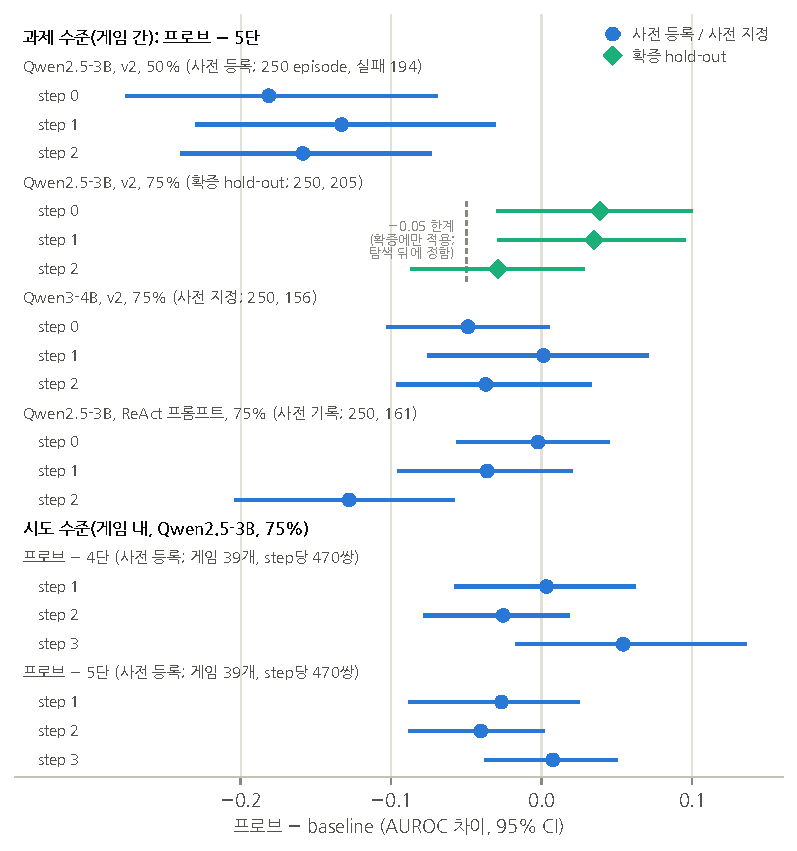
\includegraphics[width=0.82\linewidth]{fig3_probe_minus_baseline_ko.pdf}
\caption{사전 등록·사전 지정·확증 프로브 대 baseline 비교 전부(18개, 우수 0개). 이 비교들은 게임과 baseline을 공유해 독립이 아니므로, 개수는 합친 추정치가 아니다. 점은 AUROC 차이, 막대는 95\% CI. 과제 수준: 프로브 $-$ 5단, scene 단위 군집 bootstrap(1,000회), 라벨에 설정과 $n$(episode, 실패). 시도 수준: 게임 내 쌍 AUROC 차이, 게임 단위 bootstrap(1,000회). 라벨을 섞은 데이터에서 이 구간은 귀무값을 80--94\%만 포함해(\ref{sec:attempt}절) 실제보다 좁다. 점선: 비열등 한계 $-0.05$, 확증 hold-out에만 적용하며 탐색 분석 뒤에 정했다. 탐색 추정치는 넣지 않았다(그림~\ref{fig:heat}).}\label{fig:forest}
% 출처: results/probe_main_3b_primary_diff.csv, confirm_main_3b_diff.csv, task_qwen3_4b_diff_p.csv, task_react_qwen25_3b_diff_p.csv, within_game_diff.csv
\end{figure}


\subsection{다른 actor와 두 번째 프롬프트}\label{sec:actors}
사전에 정한 포함 규칙으로 다섯 모델을 파일럿했고 Qwen3-4B만 통과했다(부록 표~\ref{tab:a1}--\ref{tab:a2}). 이 모델의 프로브도 어느 라운드에서 5단을 넘지 못했고($-0.049$, $+0.001$, $-0.037$, 모두 결론 없음), 샘플링 rollout이 거의 갈라지지 않아(50게임 중 10게임) 시도 수준 질문에는 답할 수 없었다(부록 표~\ref{tab:a3}).
Qwen2.5-3B를 ReAct 원 예시~\cite{yao2023react}로 다시 돌리면(부록 표~\ref{tab:a4}) $-0.002$, $-0.036$, $-0.128$($-0.204$ \textasciitilde{} $-0.058$)로, 우수한 라운드는 없었고 step 2는 열등이었다(부록 표~\ref{tab:settings}).
과제 수준 평가 네 가지에서 프로브가 5단보다 우수한 라운드는 12개 중 0개였다. v2 궤적으로 학습한 프로브는 ReAct 궤적에 잘 옮겨 가지 않았고(0.527, 0.493, 0.555), 이는 프로브의 방향이 프롬프트 형식에 묶여 있음을 시사한다.

\subsection{선행 방식 모니터와의 비교}\label{sec:prior}
기존 에이전트 모니터의 과제를 보지 못하는 baseline을 근사하면(탐색, 부록 표~\ref{tab:prior}), 같은 프로브가 \cite{ruan2026doomed}를 따른 행동 scorer보다 $+0.145$--$+0.190$ 높았고 \cite{pham2026agentstop}를 따른 로그확률 scorer보다 step 1과 2에서 높았다.
행동 특징에 과제 유형만 더해도 AUROC가 0.08--0.10 올랐고, 5단 전체와 비교하면 프로브의 이점이 없었다. 과제를 보지 못하는 모니터 대비 hidden state의 이점은 baseline이 과제를 보면 사라질 수 있다.

\subsection{조기 중단}
100 action 상한의 탐욕 500게임에서 중단 규칙을 평가했고, 성공 손실 10\% 이하에서 절감한 step 비율의 최댓값 평균을 지표로 썼다(표~\ref{tab:early}). 프로브는 step의 0.529를, step 상한은 0.560을 절감했고, 주 비교 차이는 $-0.032$($-0.183$ \textasciitilde{} $+0.119$)로 결론 없음이었다. 이는 사전에 정한 범위에 대한 것이며, 손실 전체 범위에서는 프로브가 상한보다 더 아꼈지만($+0.056$) 5t보다는 덜 아꼈다.
보조 분석은 프로브가 고정 상한보다 나은 구간에서도 시점 맞춘 겉보기 baseline이 적어도 그만큼 낫다는 것을 시사한다(5t 0.625). 성공의 10\%가 약 11개 episode라 신뢰구간이 넓다.

% Generated by scripts/2026-10-21/extract_floats.py from paper/main_ko.tex; edit the full manuscript, not this file.
\begin{table}[htbp]
\centering\small
\caption{Early termination, Qwen2.5-3B, 500 games, 100-action horizon.}\label{tab:early}
\begin{tabularx}{\linewidth}{@{}l>{\centering\arraybackslash}Xc@{}}
\toprule
Rule & Mean max.\ steps saved at $\le$10\% lost successes (95\% CI) & Relative to oracle \\
\midrule
Step cap & 0.560 (0.468, 0.656) & 0.58 \\
Loop detector & 0.194 (0.023, 0.361) & 0.20 \\
Rung 4t & 0.608 (0.477, 0.748) & 0.63 \\
Rung 5t & 0.625 (0.503, 0.758) & 0.65 \\
Probe (75\% depth + step) & 0.529 (0.382, 0.667) & 0.55 \\
Oracle (stop failures at step 0) & 0.958 (0.947, 0.969) & 1 \\
\bottomrule
\end{tabularx}
\end{table}


\subsection{강건성}\label{sec:robust}
100 action 라벨로 바꿔도 우수한 라운드는 없었다. 더 강한 프로브 다섯 개(넓힌 정규화 격자, PCA, 네 깊이 결합, MLP 격자, 5단에 hidden state 추가)도 18개 비교 중 5단보다 우수한 것이 없었고 가장 큰 차이는 $+0.013$이었다(부록 표~\ref{tab:strength}).
사전 등록 라운드 너머 step 0--10의 차이는 $-0.114$에서 $+0.009$ 사이였고, 이전 step hidden state의 누적 평균을 쓴 프로브도 낫지 않았다. step 7부터는 4단이 프롬프트에 보이는 최근 6 step보다 오래된 action을 쓴다.
탐색 점검(앞 250개 episode와 500개 전체 sweep 하나, 분석마다 1회)에서, 학습 데이터를 늘려도 프로브 $-$ 5단이 줄어드는 것은 탐지되지 않았고(앞 250개에서 학습 약 50--200개일 때 $-0.002$ \textasciitilde{} $-0.025$, 500개 전체에서 평가 fold를 고정하고 약 50--400개일 때 $+0.016$ \textasciitilde{} $+0.006$, 변화 $-0.010$, 95\% 신뢰구간 $-0.038$ \textasciitilde{} $+0.022$로 약 0.02까지의 좁아짐은 배제하지 못하며 두 방법 모두 아직 오르는 중), 오탐률 10\%에서 프로브는 실패의 0.268을, 5단은 0.407을 검출했다(차이 $-0.139$, $-0.273$ \textasciitilde{} $+0.075$). 게임 단위 분할은 AUROC를 프로브에서 $-0.006$, 5단에서 $-0.027$만 바꿨다. action 마지막 토큰의 hidden state를 읽어도 결론은 같았고(75\% 깊이 $-$ 5단 $-0.019$, $-0.085$ \textasciitilde{} $+0.046$), 문장 인코더(bge-base-en-v1.5) 텍스트 baseline은 TF-IDF보다 약했다($-0.115$). 라벨을 섞은 데이터에서 과제 수준 구간은 귀무값을 95\%가 아니라 85--90\%만 포함했다(프로브의 90\%는 95\%와도 80\%와도 구별되지 않음). 사전 등록 구간을 1.26배 넓혀도 상한은 모두 0 아래였지만 step 1은 간신히 그랬다($-0.004$).

\section{토의}
과제 수준 평가 네 가지에서 actor hidden state의 선형 프로브는 겉보기 정보로 만든 baseline보다 나은 적이 없었고, 사전 등록 조건에서는 더 낮았다.
어느 방법이든 게임 간에 예측한 것의 대부분은 게임 자체였다. 게임 안에서는 step 2부터 실패가 보였지만, 텍스트와 진행도 특징에도 똑같이 보였다.
에이전트 hidden state의 프로브가 행동 수준 특징만 보는 모니터보다 낫다는 보고가 있다~\cite{ruan2026doomed}. 우리 결과는 과제를 보는 사다리가 그 차이를 메웠으므로 그런 비교가 hidden state의 기여를 과대평가할 수 있음을 시사한다. 다만 그들의 환경은 재현하지 않았고 프로브가 읽는 위치도 다르다(action 토큰을 읽어도 결론은 같았다, \ref{sec:robust}절).
수학 추론에서는 초기 프로브가 문제 안에서 우연 수준으로 떨어졌지만~\cite{bulut2026problem}, 우리 에이전트에서는 게임 안 신호가 우연보다 높았다. 궤적이 관찰 가능한 방식으로 갈라지고 텍스트 baseline과 프로브가 모두 이를 읽기 때문으로 보이지만 검정하지는 않았다.
웹 에이전트에서도 겉보기 신호가 내부 신호와 경쟁할 만했고~\cite{pan2026monitoring}, 가벼운 TF-IDF 감지기가 LLM 심사 모델보다 에이전트의 거짓 성공을 더 잘 찾았다~\cite{advani2026false}. 프롬프트 사이에서 프로브가 잘 옮겨 가지 않은 결과는 진실성 프로브의 기하가 프롬프트 템플릿에 따라 달라진다는 보고~\cite{poulis2026truth}와 같은 방향이다.

\paragraph{여기서 hidden state가 도움이 되지 않은 이유.} 세 가지 설명이 가능하며, 셋째만 탐색적으로 직접 살펴보았다. 첫째, 평가한 step에서는 결과가 대부분 게임으로 정해지고 프롬프트가 이미 과제와 방을 서술하므로, 프로브가 쓸 수 있는 정보는 텍스트에도 있다.
둘째, 프롬프트 사이의 약한 전이가 시사하듯 프로브가 일반적인 실패 상태가 아니라 프롬프트의 형식을 담은 방향을 배울 수 있다(두 프롬프트는 hidden state를 뽑는 토큰도 다르다).
셋째, fold당 학습 episode가 약 200개이고 차원이 2,048이라 정규화한 선형 프로브가 약할 수 있다. 다만 reader, 깊이, 프로브 종류의 탐색 조합 96개와 더 강한 프로브 다섯 개도 baseline을 넘지 못했고, 학습 episode 약 50--400개 범위에서도, 약 400--1,200개 범위에서도($-0.008$, 95\% 신뢰구간 $-0.017$ \textasciitilde{} $+0.002$, 1,500개 episode) 격차 변화가 탐지되지 않았다. 마지막 템플릿 토큰 대신 프롬프트의 다른 다섯 위치를 읽어도 75\% 깊이 AUROC는 0.727--0.749였고, 마지막 프롬프트 토큰이나 5단과 구분된 차이는 없었다(사후).

\paragraph{보완적 해석.} 75\% 깊이에서 토큰 하나를 읽고 fold당 약 200개 episode로 학습한 프로브는 공들여 만든 5단 baseline과 AUROC 0.011--0.034 차이 안에 있었고, 홀드아웃의 step 0과 1에서는 유의하지 않지만 앞섰다. 실패와 관련된 정보의 상당 부분이 표현 안에 선형으로 들어 있다는 뜻이며, 평가 행을 고정하면 학습 episode 약 50--400개와 약 400--1,200개 범위 모두에서 격차 변화가 탐지되지 않았다(후자 $-0.008$, $-0.017$ \textasciitilde{} $+0.002$). 75\% 깊이는 탐색한 깊이들을 본 뒤 고른 것이며, 사전 등록한 50\% 칸은 5단보다 0.13--0.18 낮았다.

\paragraph{실용적 함의.} 작은 에이전트가 스스로 모니터를 돌린다면 hidden state는 추가 비용이 없으므로 작은 이득이라도 쓸모가 있다. 그러나 그런 이득은 찾지 못했다. 성공 손실 10\% 이하에서 step 상한은 프로브만큼 step을 아꼈고, 겉보기 baseline은 적어도 그만큼 아꼈다.
단순한 상한이나 에이전트의 텍스트를 읽는 모니터가 더 싼 출발점이며 모델 내부에 접근할 필요도 없다.

\paragraph{방법론적 시사점.} 몇몇 설계 선택은 비슷한 연구에서 결론을 바꿀 수 있다. 방 배치가 아니라 게임 단위로 나누면 장면 정보만 담은 합성 특징의 AUROC가 0.97까지 부풀었다(실제 프로브와 5단에서는 $-0.006$, $-0.027$로 작았다).
게임 내 평가는 아직 갈라지지 않은 rollout 때문에 희석되었고(쌍의 52--70\%가 동점), 라벨을 섞은 데이터에서 게임 단위 percentile bootstrap 구간은 너무 좁았다(포함률 95\%가 아니라 80--94\%, 과제 수준은 85--90\%).
시도가 갈라지는지는 정책에 달려 있다. $T = 1$로 샘플링한 Qwen3-4B는 50게임 중 10게임에서만 갈라졌다.

\section{한계}\label{sec:limits}
환경 하나, 3--4B 크기의 Qwen 모델 2개, 프롬프트 2개만 시험했다. Qwen 이외 모델 세 개는 우리 프롬프트에서 파일럿 20게임 중 1개만 풀었는데, 이는 프롬프트와 모델의 궁합 때문일 수 있다. action은 자유 생성이 아니라 후보 점수화로 골랐다.
평가 집합마다 250개 episode라 신뢰구간이 약 $\pm$0.06--0.10이어서 작은 차이는 가릴 수 없다. 75\% 깊이와 0.05 마진은 탐색 뒤에 정했고, 시도 수준 결과는 샘플링 정책과 탐욕 결과로 고른 게임에서 나왔으며, 조기 중단 비용은 action 수로만 셌고, 7B reader는 4비트로 양자화되었다.
사전 등록 라운드는 처음 세 action뿐이다. episode를 30 action에서 끊었으며, 탐욕 실패 399개를 100 action까지 다시 돌리면 2.8\%가 늦게 성공했지만 100 action 라벨에서도 결론은 바뀌지 않았다. 주 프롬프트는 직접 작성해 데이터 수집 전에 다른 분할에서 고쳤고, 외부 프롬프트는 따로 시험했다.
TF-IDF는 약한 텍스트 baseline이며, 시험한 신경망 인코더 하나는 이보다도 약했다. 낮은 오탐 구간의 검출률은 성공 56개로 한 탐색 점검에서만 AUROC와 같은 방향이었고, 과제 수준 구간은 라벨을 섞은 데이터에서 귀무값을 85--90\%만 포함했다. 초반 상태로 도달 가능한 AUROC는 추정하지 않았다. 비교 18개는 게임과 baseline을 공유해 독립이 아니며, reader마다 hidden 차원이 다르다(896--3,584). 계획은 외부 등록처가 아니라 저장소의 날짜 있는 commit으로 등록했다(벗어난 점은 부록 표~\ref{tab:a8}). 두 번째 환경, 정식 동등성 분석, Monte Carlo value 타깃은 새 수집이나 등록하지 않은 마진이 필요해 시도하지 않았다. 약 1,200개를 넘는 학습 집합은 시도하지 않았다(추가 1,000개 episode는 표본 확대 금지 규칙의 등록된 예외).

\section{결론}
소형 Qwen 에이전트의 hidden state에 학습한 선형 프로브는 과제·프롬프트 텍스트·진행도 특징으로 만든 baseline보다 ALFWorld 실패를 더 잘 예측하지 못했다. 사전 등록 분석, 홀드아웃, 두 번째 모델, 외부 프롬프트 어디에서도 마찬가지였고, 성공 손실 10\% 이하에서 프로브로 실패할 episode를 멈추는 것이 고정 상한보다 step을 더 아낀다는 것은 보이지 않았다.
hidden state가 에이전트의 실패를 드러낸다는 주장은 같은 과제 정보를 보는 baseline과 비교하고, 과제 안에서 평가해 검증해야 한다.

\section*{코드와 데이터 공개}
코드, 설정, 각 실행 전에 고정한 분석 계획(날짜 포함), 보고한 수치를 낸 결과 표, 그림 스크립트는 공개 저장소에 있다(심사를 위해 링크 생략). 수집한 궤적과 hidden state(3.6 GB)는 용량 때문에 저장소에 없다.
% 투고처가 정해지면 정할 것: 저장소 링크(camera-ready)와 궤적·hidden state 공유 방식(예: 데이터 DOI).

\bibliographystyle{unsrtnat}
\bibliography{refs}

\clearpage
\appendix
\section{추가 결과와 사전 등록 항목}
\setcounter{table}{0}\renewcommand{\thetable}{A\arabic{table}}
\setcounter{figure}{0}\renewcommand{\thefigure}{A\arabic{figure}}
전체 방법과 모든 보조 분석은 이 논문의 전체판에 있으며, 아래 표와 그림은 전체판과 같다.

% Generated by scripts/2026-10-21/extract_floats.py from paper/main_ko.tex; edit the full manuscript, not this file.
\begin{table}[htbp]
\centering\small
\caption{Pre-registered hypothesis, decision rules and interpretation tables (wording from the frozen plans).}\label{tab:a7}
\begin{tabularx}{\linewidth}{@{}L>{\raggedright\arraybackslash}p{2.9cm}>{\raggedright\arraybackslash}p{2.9cm}@{}}
\toprule
Pre-registered item & Fixed & Observed \\
\midrule
\textbf{Task level.} H1: on 3B trajectories with the 3B reader, the probe AUROC at rounds 1--3 is higher than rung 5 (95\% CI of the difference excludes zero, above). & Before the primary run (2026-10-15) & Not supported: all three differences below zero \\
\addlinespace
Interpretation (a): only the 3B reader beats rung 5 $\rightarrow$ readable information has a size boundary. (b): all reader sizes beat it similarly $\rightarrow$ the information is at text level, so small models read it too. (c): even the 3B reader does not beat it $\rightarrow$ visible information suffices in this setting (negative result). & Before the primary run & (c) \\
\addlinespace
Decision rule for a difference: superior if the lower 95\% bound $> 0$; non-inferior if it $> -0.05$; inferior if the upper bound $< 0$; otherwise inconclusive. The 0.05 margin was set after the exploratory analysis. & Margin: after exploration, before the hold-out was evaluated & Hold-out: non-inferior, non-inferior, inconclusive (Table~\ref{tab:confirm}) \\
\addlinespace
\textbf{Attempt level.} Probe $>$ rungs 4 and 5 (lower 95\% bound $> 0$) $\rightarrow$ hidden states carry an in-progress failure signal not explained by difficulty text. Probe $\approx$ baseline $\rightarrow$ a signal exists but adds nothing beyond the history. All near 0.5 $\rightarrow$ success and failure within a game are not predicted by these methods. & Before the sampled rollouts were collected & Fits no row cleanly (Section~\ref{sec:attempt}) \\
\addlinespace
Supplementary rules for the attempt level: ``$\approx$'' only if the 95\% CI of the difference lies within $\pm 0.05$ (a lower bound above $-0.05$ alone is ``non-inferior, weak''); ``near 0.5'' if the CI includes 0.5 and the within-game permutation $p > 0.05$; Holm adjustment over the six comparisons. & Before the attempt-level results were opened (2026-10-17) & No comparison superior or equivalent \\
\bottomrule
\end{tabularx}
\par\smallskip\raggedright\footnotesize
% 출처: \code{docs/paper\_draft\_2026-10-15.md}(2절), \code{docs/multi\_rollout\_plan\_2026-10-15.md}(해석 규칙, 2026-10-17 보완 규칙). 판정 규칙은 \ref{sec:stats}절에도 적었다.
\end{table}

% Generated by scripts/2026-10-21/extract_floats.py from paper/main_ko.tex; edit the full manuscript, not this file.
\begin{table}[htbp]
\centering\small
\caption{Deviations from the registered plans and exposures to results before a decision.}\label{tab:a8}
\footnotesize\setlength{\tabcolsep}{4pt}
\begin{tabularx}{\linewidth}{@{}>{\raggedright\arraybackslash}p{2.1cm}L>{\raggedright\arraybackslash}p{2.6cm}>{\raggedright\arraybackslash}p{2.8cm}@{}}
\toprule
Plan & Change or exposure & When & Effect on reported results \\
\midrule
Task-level freeze & Sample size raised from 250 to 500 episodes to create the confirmatory hold-out; policy, prompt and code unchanged & 2026-10-15, before the hold-out was collected & Hold-out analysed as one separate comparison \\
\addlinespace
Task-level freeze & Repository history rewritten to clean commit messages; the frozen commit hash changed (tree identical, mapping kept) & 2026-10-15 & None on data or code; registration rests on dated commits and the mapping \\
\addlinespace
Confirmatory comparison & Non-inferiority margin 0.05 chosen after the exploratory analysis & Before the hold-out was evaluated & Non-inferior labels are weak (Table~\ref{tab:confirm} note) \\
\addlinespace
Attempt level & Games stratified by greedy outcome, decided after the pilot & Before the main set was collected & Variance explained by the game is not a population value \\
\addlinespace
Attempt level & Supplementary analyses and interpretation rules added (equivalence band, near-0.5 rule, Holm adjustment) & 2026-10-17, before the results were opened & Primary verdicts reported unchanged; rules applied in addition \\
\addlinespace
Attempt level & Another session saw the first two lines of the results log (run size and the $\eta^2$ point estimate) & Before the attempt-level results were opened & Reported; no other result was seen \\
\addlinespace
100-action re-run & Interim counts seen twice during collection (3 late successes among the first 116 games); a partial collection was discarded after a shutdown & 2026-10-17, before the decision & Decision rule unchanged (committed beforehand) \\
\addlinespace
Early termination & Loop-detector definition clarified, then corrected so that the count excludes the action itself & 2026-10-20, before code was run and results opened & None on the other rules \\
\addlinespace
Model extension & Inclusion rule changed so that every model passing the pilot criteria enters & 2026-10-20, before the SmolLM3 pilot & Substitutes cannot be chosen after results; no further models added \\
\addlinespace
Model pilots & Reference time of the time criterion was not defined; judged against a reference value & 2026-10-17, after the first pilots & Exclusions rest on the success criterion \\
\addlinespace
Second prompt (ReAct) & Methods of the secondary success-rate comparison (Wilson CI, game-level bootstrap, exact McNemar) were not in the plan & 2026-10-20, fixed in the script before running & Secondary result only \\
\addlinespace
Additional checks & Six exploratory checks (training-set size, low false-positive region, split unit, interval coverage, action-token position, text encoder) planned after the pre-registered, confirmatory and exploratory results had been read & 2026-10-21, plan fixed before each check was run & Exploratory only; no verdict changed \\
\addlinespace
Training-size sweep & Sweep on all 500 episodes reuses the confirmatory hold-out for training and evaluation; planned after the first-250 learning curve and the hold-out results had been read & 2026-10-21, plan fixed before the run & Exploratory only; the confirmatory verdict is unchanged \\
\addlinespace
Training-size sweep (1,500 episodes) & 1,000 new greedy episodes collected as an exception to the rule against enlarging samples; plan (sizes, primary contrast, interpretation rules) planned after the 500-episode sweep and the earlier results had been read & 2026-10-21, approved before collection & Exploratory only; the confirmatory verdict is unchanged \\
\addlinespace
Training-size sweep (1,500 episodes) & Plan extended by an equivalence-margin table (0.02, 0.05, 0.10) and an evaluation on the 1,000 new episodes only, in anticipation of review questions; no margin was registered & 2026-10-23, before the new data were analysed & Descriptive; primary contrast and interpretation rules unchanged \\
\addlinespace
Exposure during collection & The win/loss lines of an interrupted collection of 39 episodes (discarded) were seen in command output; later the win count of the first 251 new episodes and the overall success rate (0.208) were seen in the same way; none was an analysis input & 2026-10-23; the first before, the other two after the plan extension above & Primary contrast and interpretation rules unchanged \\
\addlinespace
Training-size sweep (1,500 episodes) & The first run of the analysis (2026-10-23) was interrupted and produced no output; it was run again with unchanged code, data and procedure, and no result of the first run had been seen & 2026-10-24 & None \\
\addlinespace
Comparison with rung 4 & Intervals for probe minus rung 4 and rung 5 minus rung 4 added after the sweep results had been read; same procedure, scores recomputed (matching the sweep to $10^{-16}$) & 2026-10-24, plan note written before the run & Exploratory only and uncorrected; primary verdict unchanged \\
\bottomrule
\end{tabularx}
\par\smallskip\raggedright\footnotesize
계획 문서들의 변경 이력에서 모았다. 본문에 이미 적은 항목도 한곳에서 보이도록 다시 실었다.
\end{table}

% Generated by scripts/2026-10-21/extract_floats.py from paper/main_ko.tex; edit the full manuscript, not this file.
\begin{table}[htbp]
\centering\small
\caption{Confirmatory hold-out (episodes 250--499; 3B reader, 75\% depth, linear).}\label{tab:confirm}
\begin{tabularx}{\linewidth}{@{}Lccc@{}}
\toprule
 & Step 0 & Step 1 & Step 2 \\
\midrule
Probe AUROC (95\% CI) & 0.645 (0.547, 0.736) & 0.716 (0.619, 0.810) & 0.729 (0.633, 0.815) \\
Rung 5 AUROC & 0.607 & 0.681 & 0.758 \\
Probe $-$ rung 5 (95\% CI) & $+0.039$ ($-0.030$, $+0.100$) & $+0.035$ ($-0.030$, $+0.096$) & $-0.029$ ($-0.087$, $+0.029$) \\
Decision (margin 0.05, set post hoc) & non-inferior & non-inferior & inconclusive \\
\bottomrule
\end{tabularx}
\par\smallskip\raggedright\footnotesize
$n = 250$ episodes (205 failures). Training used all 500 episodes; evaluation used only the new 250. 마진 민감도(같은 신뢰구간으로 읽음; 하한 $-0.030$, $-0.030$, $-0.087$, 상한은 모두 0 위): 마진 0.025이면 비열등인 step이 없고, 0.10이면 세 step 모두 비열등이다. 마진을 사후에 정했으므로 근거는 판정 라벨이 아니라 차이와 신뢰구간이다.
\end{table}

% Generated by scripts/2026-10-21/extract_floats.py from paper/main_ko.tex; edit the full manuscript, not this file.
\begin{table}[htbp]
\centering\small
\caption{Task-level probe $-$ rung 5 (AUROC difference, 95\% CI) across settings.}\label{tab:settings}
\begin{tabularx}{\linewidth}{@{}Lccc@{}}
\toprule
Setting & Step 0 & Step 1 & Step 2 \\
\midrule
Qwen2.5-3B, v2, 50\% depth (pre-registered; $n = 250$, 194 failures) & $-0.181$ ($-0.276$, $-0.069$) & $-0.133$ ($-0.230$, $-0.031$) & $-0.159$ ($-0.240$, $-0.073$) \\
Qwen2.5-3B, v2, 75\% depth (confirmatory hold-out; 250, 205) & $+0.039$ ($-0.030$, $+0.100$) & $+0.035$ ($-0.030$, $+0.096$) & $-0.029$ ($-0.087$, $+0.029$) \\
Qwen3-4B, v2, 75\% depth (pre-specified; 250, 156) & $-0.049$ ($-0.103$, $+0.005$) & $+0.001$ ($-0.076$, $+0.071$) & $-0.037$ ($-0.096$, $+0.033$) \\
Qwen2.5-3B, ReAct prompt, 75\% depth (pre-recorded; 250, 161) & $-0.002$ ($-0.057$, $+0.045$) & $-0.036$ ($-0.096$, $+0.021$) & $-0.128$ ($-0.204$, $-0.058$) \\
\bottomrule
\end{tabularx}
\par\smallskip\raggedright\footnotesize
프로브와 5단 AUROC: Qwen3-4B 0.660/0.687/0.680 대 0.709/0.686/0.717, ReAct 프롬프트 0.659/0.623/0.593 대 0.661/0.660/0.721. 장면 단위 cluster bootstrap 1,000회.
\end{table}

% Generated by scripts/2026-10-21/extract_floats.py from paper/main_ko.tex; edit the full manuscript, not this file.
\begin{figure}[htbp]
\centering
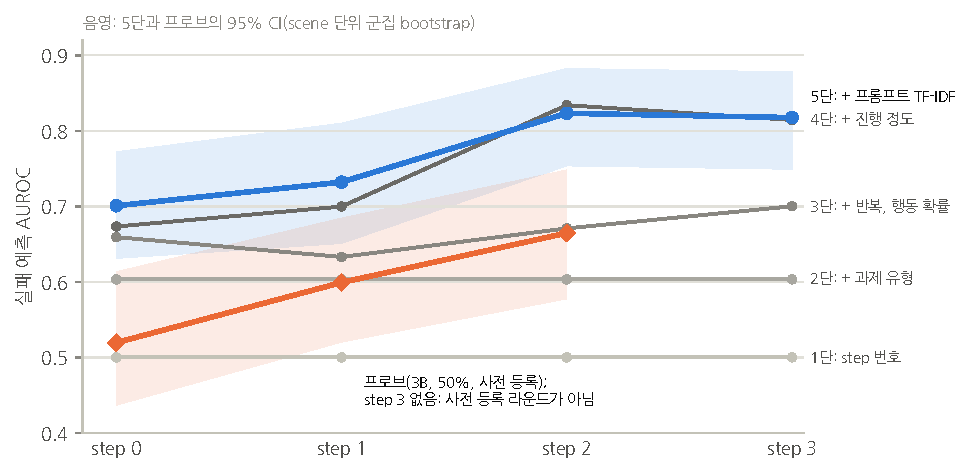
\includegraphics[width=\linewidth]{fig2_baseline_ladder_ko.pdf}
\caption{처음 250 episode에서 baseline 사다리(step 0--3)와 사전 등록 프로브(step 0--2)의 실패 예측 AUROC(step마다 $n = 250$, 실패 194). 5단과 프로브를 강조하고 scene 단위 군집 bootstrap(1,000회) 95\% CI를 음영으로 표시했다. 1--4단의 CI는 가독성을 위해 생략했다. 1단은 설계상 0.5이고 2단은 step에 따라 변하지 않는다. 두 음영이 겹치는지는 차이의 검정이 아니며, 짝지은 차이는 그림~\ref{fig:forest}에 있다.}\label{fig:ladder}
% 출처: results/baselines_main_3b.csv, results/probe_main_3b_primary.csv
\end{figure}

% Generated by scripts/2026-10-21/extract_floats.py from paper/main_ko.tex; edit the full manuscript, not this file.
\begin{figure}[htbp]
\centering
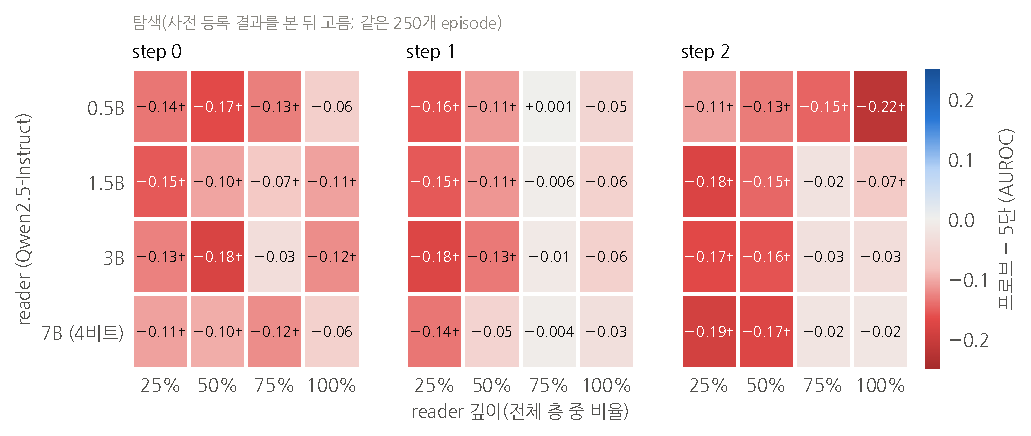
\includegraphics[width=\linewidth]{fig4_reader_depth_ko.pdf}
\caption{탐색: 처음 250 episode에서 선형 프로브의 모든 reader $\times$ 깊이 조합의 프로브 $-$ 5단 AUROC 차이(48칸, 선택 없음). 0을 중심으로 한 발산 색(빨강: 프로브가 5단보다 낮음). $\dagger$는 95\% CI(scene 단위 군집 bootstrap)가 0을 포함하지 않는 칸이며 모두 0 아래다(48칸 중 31칸). CI가 0 위에 있는 칸은 없고 가장 큰 차이는 $+0.001$이다. 7B reader는 4비트 가중치를 써서 크기와 양자화가 섞여 있다. MLP 칸과 CI: 부록 표~\ref{tab:a6}.}\label{fig:heat}
% 출처: results/explore_{0.5B,1.5B,3B,7B-4bit}_diff.csv
\end{figure}

% Generated by scripts/2026-10-21/extract_floats.py from paper/main_ko.tex; edit the full manuscript, not this file.
\begin{table}[htbp]
\centering\small
\caption{Exploratory: linear-probe AUROC by reader and depth, first 250 episodes, mean over steps 0--2.}\label{tab:a6}
\begin{tabularx}{\linewidth}{@{}lccccL@{}}
\toprule
Reader & 25\% & 50\% & 75\% & 100\% & Probe $-$ rung 5, all 24 cells per reader (min, max) \\
\midrule
0.5B & 0.618 & 0.615 & \textbf{0.660} & 0.642 & $-0.277$, $+0.001$ \\
1.5B & 0.589 & 0.631 & \textbf{0.717} & 0.675 & $-0.195$, $-0.006$ \\
3B (= actor) & 0.595 & 0.594 & \textbf{0.727} & 0.682 & $-0.205$, $+0.004$ \\
7B (4-bit) & 0.608 & 0.643 & 0.704 & \textbf{0.717} & $-0.191$, $-0.004$ \\
\bottomrule
\end{tabularx}
\par\smallskip\raggedright\footnotesize
5단은 step 0--2 평균 0.752였다. 마지막 열은 네 깊이·세 step의 선형·MLP 프로브를 모두 포함한다(reader당 24칸, 모두 96칸). 굵은 글씨는 reader별 최고 깊이이다. 3B reader 50\% 깊이가 사전 등록 조건이다(표~\ref{tab:ladder}). 96칸 모두의 차이와 95\% CI는 표~\ref{tab:a9}에 있다.
% 출처: results/explore_{0.5B,1.5B,3B,7B-4bit}.csv, *_diff.csv
\end{table}

% Generated by scripts/2026-10-21/extract_floats.py from paper/main_ko.tex; edit the full manuscript, not this file.
\begin{table}[htbp]
\centering\scriptsize
\setlength{\tabcolsep}{3pt}
\caption{Exploratory: probe $-$ rung 5 AUROC difference (95\% CI) for all 96 cells (4 readers $\times$ 2 probe types $\times$ 4 depths $\times$ 3 steps), first 250 episodes.}\label{tab:a9}
\begin{tabular}{@{}lllccc@{}}
\toprule
Reader & Probe & Depth & Step 0 & Step 1 & Step 2 \\
\midrule
0.5B reader & Linear & 25\% & $-0.136$ ($-0.236$, $-0.037$) & $-0.159$ ($-0.253$, $-0.061$) & $-0.106$ ($-0.191$, $-0.012$) \\
0.5B reader & Linear & 50\% & $-0.168$ ($-0.273$, $-0.065$) & $-0.112$ ($-0.223$, $-0.010$) & $-0.133$ ($-0.209$, $-0.049$) \\
0.5B reader & Linear & 75\% & $-0.130$ ($-0.212$, $-0.054$) & $+0.001$ ($-0.085$, 0.087) & $-0.148$ ($-0.229$, $-0.067$) \\
0.5B reader & Linear & 100\% & $-0.062$ ($-0.130$, 0.002) & $-0.050$ ($-0.125$, 0.029) & $-0.218$ ($-0.299$, $-0.131$) \\
0.5B reader & MLP & 25\% & $-0.259$ ($-0.386$, $-0.124$) & $-0.190$ ($-0.283$, $-0.078$) & $-0.277$ ($-0.373$, $-0.168$) \\
0.5B reader & MLP & 50\% & $-0.160$ ($-0.245$, $-0.083$) & $-0.160$ ($-0.272$, $-0.044$) & $-0.144$ ($-0.216$, $-0.063$) \\
0.5B reader & MLP & 75\% & $-0.163$ ($-0.242$, $-0.090$) & $-0.068$ ($-0.155$, 0.021) & $-0.154$ ($-0.232$, $-0.077$) \\
0.5B reader & MLP & 100\% & $-0.100$ ($-0.177$, $-0.025$) & $-0.012$ ($-0.096$, 0.075) & $-0.151$ ($-0.235$, $-0.071$) \\
1.5B reader & Linear & 25\% & $-0.155$ ($-0.231$, $-0.079$) & $-0.155$ ($-0.237$, $-0.075$) & $-0.179$ ($-0.274$, $-0.084$) \\
1.5B reader & Linear & 50\% & $-0.104$ ($-0.178$, $-0.032$) & $-0.113$ ($-0.201$, $-0.020$) & $-0.146$ ($-0.231$, $-0.066$) \\
1.5B reader & Linear & 75\% & $-0.074$ ($-0.154$, $-0.006$) & $-0.006$ ($-0.074$, 0.071) & $-0.025$ ($-0.097$, 0.047) \\
1.5B reader & Linear & 100\% & $-0.105$ ($-0.188$, $-0.024$) & $-0.055$ ($-0.129$, 0.023) & $-0.069$ ($-0.135$, $-0.004$) \\
1.5B reader & MLP & 25\% & $-0.173$ ($-0.261$, $-0.080$) & $-0.170$ ($-0.247$, $-0.094$) & $-0.161$ ($-0.241$, $-0.081$) \\
1.5B reader & MLP & 50\% & $-0.195$ ($-0.293$, $-0.086$) & $-0.074$ ($-0.163$, 0.017) & $-0.138$ ($-0.232$, $-0.058$) \\
1.5B reader & MLP & 75\% & $-0.167$ ($-0.240$, $-0.089$) & $-0.086$ ($-0.177$, 0.003) & $-0.069$ ($-0.135$, $-0.003$) \\
1.5B reader & MLP & 100\% & $-0.091$ ($-0.174$, $-0.007$) & $-0.097$ ($-0.185$, $-0.003$) & $-0.121$ ($-0.208$, $-0.035$) \\
3B reader (= actor) & Linear & 25\% & $-0.127$ ($-0.206$, $-0.061$) & $-0.176$ ($-0.269$, $-0.080$) & $-0.169$ ($-0.244$, $-0.087$) \\
3B reader (= actor) & Linear & 50\% & $-0.181$ ($-0.276$, $-0.069$) & $-0.133$ ($-0.230$, $-0.031$) & $-0.159$ ($-0.240$, $-0.073$) \\
3B reader (= actor) & Linear & 75\% & $-0.034$ ($-0.102$, 0.037) & $-0.011$ ($-0.082$, 0.061) & $-0.029$ ($-0.091$, 0.027) \\
3B reader (= actor) & Linear & 100\% & $-0.120$ ($-0.196$, $-0.056$) & $-0.057$ ($-0.147$, 0.032) & $-0.034$ ($-0.098$, 0.027) \\
3B reader (= actor) & MLP & 25\% & $-0.163$ ($-0.245$, $-0.075$) & $-0.153$ ($-0.259$, $-0.048$) & $-0.205$ ($-0.292$, $-0.105$) \\
3B reader (= actor) & MLP & 50\% & $-0.198$ ($-0.295$, $-0.106$) & $-0.189$ ($-0.290$, $-0.089$) & $-0.145$ ($-0.227$, $-0.063$) \\
3B reader (= actor) & MLP & 75\% & $+0.004$ ($-0.050$, 0.061) & 0.000 ($-0.069$, 0.069) & $-0.036$ ($-0.098$, 0.025) \\
3B reader (= actor) & MLP & 100\% & $-0.095$ ($-0.168$, $-0.025$) & $-0.057$ ($-0.145$, 0.031) & $-0.038$ ($-0.097$, 0.021) \\
7B reader (4-bit) & Linear & 25\% & $-0.107$ ($-0.208$, $-0.005$) & $-0.136$ ($-0.215$, $-0.051$) & $-0.189$ ($-0.277$, $-0.104$) \\
7B reader (4-bit) & Linear & 50\% & $-0.099$ ($-0.177$, $-0.019$) & $-0.053$ ($-0.141$, 0.032) & $-0.175$ ($-0.251$, $-0.097$) \\
7B reader (4-bit) & Linear & 75\% & $-0.119$ ($-0.189$, $-0.048$) & $-0.004$ ($-0.094$, 0.093) & $-0.021$ ($-0.080$, 0.046) \\
7B reader (4-bit) & Linear & 100\% & $-0.058$ ($-0.141$, 0.022) & $-0.030$ ($-0.113$, 0.056) & $-0.017$ ($-0.080$, 0.050) \\
7B reader (4-bit) & MLP & 25\% & $-0.154$ ($-0.251$, $-0.051$) & $-0.132$ ($-0.232$, $-0.028$) & $-0.144$ ($-0.229$, $-0.060$) \\
7B reader (4-bit) & MLP & 50\% & $-0.191$ ($-0.286$, $-0.096$) & $-0.122$ ($-0.221$, $-0.021$) & $-0.149$ ($-0.226$, $-0.072$) \\
7B reader (4-bit) & MLP & 75\% & $-0.124$ ($-0.216$, $-0.036$) & $-0.079$ ($-0.162$, 0.011) & $-0.094$ ($-0.170$, $-0.020$) \\
7B reader (4-bit) & MLP & 100\% & $-0.071$ ($-0.158$, 0.012) & $-0.087$ ($-0.177$, 0.001) & $-0.039$ ($-0.115$, 0.031) \\
\bottomrule
\end{tabular}
\par\smallskip\raggedright\footnotesize
장면 단위 cluster bootstrap 1,000회. step당 $n = 250$(실패 194). 7B reader는 4비트 가중치를 썼다. 3B reader의 50\% 깊이 선형 칸이 사전 등록 조건이다.
% Source: results/explore_{0.5B,1.5B,3B,7B-4bit}_diff.csv
\end{table}

% Generated by scripts/2026-10-21/extract_floats.py from paper/main_ko.tex; edit the full manuscript, not this file.
\begin{table}[htbp]
\centering\small
\caption{Exploratory: task-level AUROC of prior-style baselines, first 250 episodes.}\label{tab:prior}
\begin{tabularx}{\linewidth}{@{}Lccc@{}}
\toprule
 & Step 0 & Step 1 & Step 2 \\
\midrule
Behavioral features (after~\cite{ruan2026doomed}) & 0.522 & 0.554 & 0.605 \\
Log-probability features (after~\cite{pham2026agentstop}) & 0.626 & 0.545 & 0.606 \\
Behavioral + task type & 0.626 & 0.656 & 0.689 \\
Rung 5 & 0.701 & 0.732 & 0.823 \\
Probe (75\% depth, linear) & 0.666 & 0.721 & 0.795 \\
\addlinespace
Probe $-$ behavioral (95\% CI) & $+0.145$ (0.032, 0.247) & $+0.167$ (0.070, 0.247) & $+0.190$ (0.107, 0.282) \\
Probe $-$ log-probability (95\% CI) & $+0.040$ ($-0.060$, 0.133) & $+0.176$ (0.051, 0.297) & $+0.189$ (0.074, 0.296) \\
Probe $-$ rung 5 (95\% CI) & $-0.034$ ($-0.102$, 0.037) & $-0.011$ ($-0.082$, 0.061) & $-0.029$ ($-0.091$, 0.027) \\
\bottomrule
\end{tabularx}
\par\smallskip\raggedright\footnotesize
step당 $n = 250$(실패 194). 장면 단위 cluster bootstrap 1,000회.
% 출처: results/prior_methods_3b*.csv
\end{table}

% Generated by scripts/2026-10-21/extract_floats.py from paper/main_ko.tex; edit the full manuscript, not this file.
\begin{table}[htbp]
\centering\small
\caption{Exploratory: stronger probes $-$ rung 5 (AUROC difference, 95\% CI), first 250 episodes.}\label{tab:strength}
\begin{tabularx}{\linewidth}{@{}Lccc@{}}
\toprule
Probe & Step 0 & Step 1 & Step 2 \\
\midrule
Reference (75\% depth, linear, $C \le 1$) & $-0.034$ ($-0.102$, 0.037) & $-0.011$ ($-0.082$, 0.061) & $-0.029$ ($-0.091$, 0.027) \\
Wider $C$ grid & $-0.036$ ($-0.105$, 0.036) & $+0.013$ ($-0.072$, 0.101) & $-0.034$ ($-0.099$, 0.026) \\
PCA ($k$ 8--128) & $-0.019$ ($-0.084$, 0.041) & $-0.037$ ($-0.103$, 0.032) & $-0.029$ ($-0.091$, 0.026) \\
Four depths concatenated & $-0.052$ ($-0.121$, 0.008) & $-0.055$ ($-0.127$, 0.023) & $-0.077$ ($-0.159$, $-0.003$) \\
MLP (grid of 4) & $-0.036$ ($-0.104$, 0.023) & $-0.025$ ($-0.105$, 0.058) & $-0.052$ ($-0.122$, 0.017) \\
Rung 5 + hidden state & $-0.034$ ($-0.101$, 0.037) & $-0.023$ ($-0.096$, 0.047) & $-0.024$ ($-0.086$, 0.032) \\
\bottomrule
\end{tabularx}
\par\smallskip\raggedright\footnotesize
5단 AUROC 0.701, 0.732, 0.823. step당 $n = 250$(실패 194). 장면 단위 cluster bootstrap 1,000회.
% 출처: results/probe_strength_3b*.csv, results/extra_main_3b_B_late_rounds.csv, results/extra_main_3b_C_temporal.csv
\end{table}

% Generated by scripts/2026-10-21/extract_floats.py from paper/main_ko.tex; edit the full manuscript, not this file.
\begin{table}[htbp]
\centering\small
\caption{Model pilots (first 20 games, v2 prompt, candidate scoring, 30 actions).}\label{tab:a1}
\footnotesize\setlength{\tabcolsep}{4pt}
\begin{tabularx}{\linewidth}{@{}L>{\centering\arraybackslash}p{2.2cm}c>{\centering\arraybackslash}p{1.6cm}>{\raggedright\arraybackslash}p{2.6cm}@{}}
\toprule
Model & Successes (Wilson 95\% CI) & s / episode & Peak GPU memory & Decision \\
\midrule
Qwen3-4B (thinking off) & 7/20 (18--57\%) & 14.9 & 10.24\,GB & included \\
Qwen3-1.7B (thinking off) & 1/20 (1--24\%) & 8.5 & 5.03\,GB & excluded (successes) \\
Llama-3.2-3B-Instruct & 1/20 (1--24\%) & 10.7 & 8.06\,GB & excluded (successes) \\
SmolLM3-3B & 1/20 (1--24\%) & 10.4 & 7.41\,GB & excluded (successes) \\
Phi-3.5-mini-instruct (candidates scored in batches of 4) & 1/20 (1--24\%) & 67.6 & 10.75\,GB & excluded (successes, time) \\
\bottomrule
\end{tabularx}
\par\smallskip\raggedright\footnotesize
같은 게임에서 Qwen2.5-3B는 5/20이었다(참고). 모든 실행이 끝까지 돌았고, 모든 action이 가능한 action이었으며, hidden state에 NaN·inf가 없었다. revision을 고정했고 chat template의 날짜도 고정했다(Llama ``26 Jul 2024'', SmolLM3 ``20 October 2026'').
\end{table}

% Generated by scripts/2026-10-21/extract_floats.py from paper/main_ko.tex; edit the full manuscript, not this file.
\begin{table}[htbp]
\centering\small
\caption{Exploratory: action patterns on the 20 pilot games.}\label{tab:a2}
\footnotesize\setlength{\tabcolsep}{4pt}
\begin{tabularx}{\linewidth}{@{}lc>{\centering\arraybackslash}p{2.2cm}>{\centering\arraybackslash}p{1.8cm}L@{}}
\toprule
Model & Successes & Repeated within last 6 steps & Distinct-action ratio & Most frequent verbs \\
\midrule
Qwen2.5-3B & 5/20 & 51\% & 0.44 & go 67\%, take 11\%, move 8\% \\
Qwen3-4B & 7/20 & 32\% & 0.54 & go 60\%, examine 14\%, open 9\% \\
Llama-3.2-3B & 1/20 & 66\% & 0.26 & examine 47\%, go 28\%, open 12\% \\
SmolLM3-3B & 1/20 & 82\% & 0.19 & examine 57\%, take 15\%, move 14\% \\
Phi-3.5-mini & 1/20 & 76\% & 0.25 & take 33\%, move 30\%, go 16\% \\
\bottomrule
\end{tabularx}
\end{table}

% Generated by scripts/2026-10-21/extract_floats.py from paper/main_ko.tex; edit the full manuscript, not this file.
\begin{table}[htbp]
\centering\small
\caption{Qwen3-4B within-game pairwise AUROC ($T = 1$ sampling; 10 of 50 games with both outcomes, 120 pairs per step).}\label{tab:a3}
\begin{tabularx}{\linewidth}{@{}Lccc@{}}
\toprule
 & Step 1 & Step 2 & Step 3 \\
\midrule
Probe (own hidden state, 75\% depth, linear) & 0.471 (0.396, 0.500) & 0.471 (0.397, 0.509) & 0.479 (0.402, 0.517) \\
Rung 4 & 0.479 (0.404, 0.519) & 0.471 (0.397, 0.509) & 0.521 (0.443, 0.611) \\
Rung 5 & 0.471 (0.391, 0.508) & 0.471 (0.397, 0.509) & 0.521 (0.443, 0.611) \\
Probe $-$ rung 4 (95\% CI) & $-0.008$ ($-0.020$, 0.000) & 0.000 (0.000, 0.000) & $-0.042$ ($-0.202$, $+0.063$) \\
Probe $-$ rung 5 (95\% CI) & 0.000 ($-0.011$, $+0.015$) & 0.000 (0.000, 0.000) & $-0.042$ ($-0.202$, $+0.063$) \\
Within-game permutation $p$, probe & 1.00 & 0.94 & 0.92 \\
\bottomrule
\end{tabularx}
\par\smallskip\raggedright\footnotesize
게임 단위 bootstrap(1,000회). $\eta^2 = 0.849$(0.747--0.935), 합친 행에서 난이도 오라클 단독 0.911. 쌍 대부분이 동점(같은 프롬프트)이라 이 값들은 정보가 적으며, 결과를 읽기 전에 정한 대로 결론을 내지 않는다(\ref{sec:actors}절).
% 출처: results/within_game_qwen3_4b*.csv
\end{table}

% Generated by scripts/2026-10-21/extract_floats.py from paper/main_ko.tex; edit the full manuscript, not this file.
\begin{table}[htbp]
\centering\small
\caption{The two prompts.}\label{tab:a4}
\begin{tabularx}{\linewidth}{@{}lLL@{}}
\toprule
 & v2 (ours) & ReAct exemplars (minimally edited) \\
\midrule
Source & Written by us; earlier version in ReAct thought--action format; frozen before data collection & Yao et al.\ (2023), \code{alfworld\_3prompts.json}, repository commit \code{6bdb3a1} \\
Format & Chat template (system + user message) & Raw completion text ending in \code{>} \\
Instructions & Six rules & One header line \\
Exemplars & One handwritten episode (clean task), same for all tasks & Two original episodes matched to the current task type, including \code{think:} lines \\
History & Last six steps & Full episode \\
Admissible actions in prompt & Yes, plus recently failed actions & No (scoring still restricted to admissible actions) \\
Scored continuation & \code{Action: a<|im\_end|>} & \code{\textvisiblespace a\textbackslash n} \\
Hidden-state token & Last token of the generation prompt & Final \code{>} \\
Edits & -- & \code{put A in/on B} $\rightarrow$ \code{move A to B} and the matching observation \\
Length (Qwen2.5 tokens) & median 864 (whole prompt) & 1,115--1,571 (exemplars only) \\
\bottomrule
\end{tabularx}
\end{table}

% Generated by scripts/2026-10-21/extract_floats.py from paper/main_ko.tex; edit the full manuscript, not this file.
\begin{table}[htbp]
\centering\small
\caption{Preliminary runs before the policy was fixed (2026-10-08).}\label{tab:a5}
\begin{tabularx}{\linewidth}{@{}Lccc@{}}
\toprule
Run & Episodes & Successes & Admissible actions \\
\midrule
Free generation, first prompt (Thought/Action), 0.5B & 2 & 0 & 8\% \\
Free generation, first prompt, 1.5B & 5 & 0 & 56\% \\
Free generation, first prompt, 3B & 5 & 1 & 61\% \\
Free generation, 1.5B, first code on the GPU machine & 3 & 0 & 26\% \\
Free generation, 1.5B, revised prompt (rules and example) & 5 & 0 & 22\% \\
Candidate scoring (final policy), 0.5B / 1.5B / 3B, training games & 20 / 100 / 100 & 0 / 2 / 20 & 100\% by construction \\
\bottomrule
\end{tabularx}
\par\smallskip\raggedright\footnotesize
자유 생성 실행은 프롬프트를 동결하기 전에 ALFWorld train 게임에서 Qwen2.5-Instruct 모델로 했다. episode가 매우 적어, 목록에 없는 action이 자주 나왔다는 것만 보여 준다. 출처: 2026-10-08 프로젝트 기록. 실행 원 로그는 저장소와 그 백업 어디에도 남아 있지 않다.
\end{table}


\end{document}
